\section{Analysis}

\subsection{Algorithm selection}

To select algorithm I use the simulated dataset. This dataset contains the latent response variable (the Sharpe ratio of each stock). We evaluate algorithm by the lowest \textit{mean squared error (mse)} of Sharpe ratios.

\begin{equation}\label{eq:meansquarederror}
    mse = \sum_{t=1}^{T} \sum_{i=1}^{k}\lp \hat{sr}_{i}^{(t)} - sr_{i}^{(t)} \rp^2
\end{equation}

The algorithm with the lowest $mse$ is the algorithm selected to be tested on real data. Before testing each algorithm we need to tune, and in the case of the $LSTM$ train the algorithm. Training the algorithm consists of tuning the parameters that are endogenous to the algorithm, and tuning consists of finding the correct values for the hyper parameters.

The LSTM is trained by splitting the dataset into two separate parts (a training set and validation set). The LSTM is trained for 4 epochs, which is the number of times the LSTM goes through the entire training data.

The Naive Rolling Sharpe is tuned on 5000 observations, where a grid search over $h= \{50, 100, 150, 200, 250, 300\}$ is used. The $h$ which corresponds to lowest $mse$ is used for the final evaluation between the algorithms. We find that $h=200$ is the best hyper parameter value for the Naive Rolling Sharpe.

The Rolling Sharpe needs the three hyper parameters: $ h_{\text{long term}}$, $h_{\text{short term}}, \tau$. We create a grid of $3^3=27$ different values as shown in equation \ref{eq:rs_grid}. The algorithm is tuned over this grid, and we find the best hyper parameters to be $h_{\text{short term}} = 30, h_{\text{long term}} = 150, \tau = 30 $.

\begin{equation}\label{eq:rs_grid}
    grid = \underset{\tau}{\{0.3, 0.5, 0.8\}} \times \underset{h_{\text{long term}}}{\{50, 100, 150\}} \times \underset{h_{\text{short term}}}{\{15, 30, 45\}}
\end{equation}

Comparing the three trained and tuned algorithms on the same $5000$ observations yields: $MSE_{\text{LSTM}}= 0.0156$, $MSE_{\text{RS}_{naive}}= 0.0181$, $MSE_{\text{RS}}= 0.0131$. We conclude that the Rolling Sharpe algorithm performs the best. In the appendix figure \ref{fig:rollingsharptest} shows the underlying true Sharpe ratio for a given stock and the corresponding prediction made by the rolling Sharpe algorithm.


\subsection{Performance on real data}

Before applying the Rolling Sharpe algorithm on the real data, a couple of benchmark is established. The \textit{perfect stock pick} benchmark, is made by assuming that we as trader had perfect foresight over the next period, and was able to pick the stock in each period which yields the highest return. The second benchmark is the \textit{Apple} stock (with ticker \textbf{AAPL}). The Apple stock is chosen, since this is the stock with the highest individual Sharpe ratio of all the stocks throughout the period. The last benchmarks are two different tangency portfolios. One based on the first 1000 observations, and a tangency portfolio based on the entire period.

Equation \ref{eq:tangencyport} displays the formula for the tangency portfolio, where $\w$ is the weights of the portfolio, and: $\mu_{adj} = \mu - \bar{r}\cdot \mathbf{1}$. Which is the risk adjusted return. It should be noted that $\w$ is a vector of length $k$ and $\sum_{w \in \w} w = 1$.

\begin{equation}\label{eq:tangencyport}
    \w = \frac{\Omega^{-1} \cdot \mu_{adj}}{\mathbf{1}^{T} \cdot \Omega^{-1} \cdot \mu_{adj}}
\end{equation}

Looking to table \ref{tab:performance} we find that the rolling Sharpe algorithm performs very well. Comparing to \textbf{Apple} we find that the sharp ratio is 4 times higher, and the expected returns is over twice as high, and a somewhat lower standard deviation. Comparing to the tangency portfolio compared over the entire period we find the Sharpe ratio to be twice as high for the rolling Sharpe algorithm. The standard deviation of the tangency portfolio is lower than that of the rolling Sharpe algorithm. However that expected return from the rolling Sharpe algorithm is almost 4 times higher. Lastly comparing to tangency portfolio of only the first 1000 observations, which more realistically would represent how an investor would generate portfolio weights, i.e. the investor cannot use the future innovations of the data generating process to construct portfolio weights. Here again we find that the rolling Sharpe algorithm has 4 times as high Sharpe ratio.

\begin{table}[ht]
\centering
\caption{Summary statistics of performance of different portfolios}
\begin{tabular}{lrrr}
\toprule
{} &  Expected Return &      Std &  Sharpe Ratio \\
\midrule
rolling sharpe                &          0.00263 &  0.02028 &       0.12562 \\
perfect stock pick            &          0.02515 &  0.02285 &       1.09734 \\
apple                         &          0.00111 &  0.02824 &       0.03661 \\
tangency portfolio (1000 obs) &          0.00058 &  0.01830 &       0.02719 \\
tangency portfolio (all obs)  &          0.00077 &  0.01246 &       0.05545 \\
\bottomrule
\end{tabular}

\label{tab:performance}
\end{table}

Figure \ref{fig:loginvest} displays (the log transformed) portfolio given one had invested following the different benchmarks, using the real data. We see again that the rolling Sharpe ratio is by far the best way to invest throughout the period. Interestingly the poorest performing portfolio is the tangency portfolio calculated on the first 1000 observations.

\begin{figure}[ht]
\centering
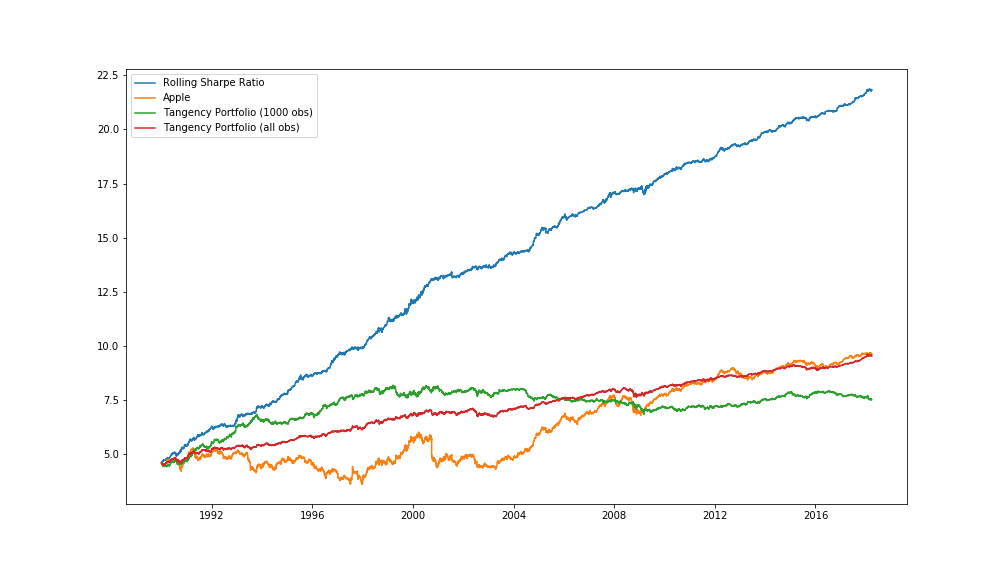
\includegraphics[scale=0.45]{figures/log_investment_experiment.png}
\caption{Counter factual portfolio performance (in logs)}
\label{fig:loginvest}
\end{figure}

Figure \ref{fig:logmontecarlo} uses Monte Carlo simulation to compare the different algorithms. By assuming that returns are normal distributed, we simulate portfolios following each of the four strategies: \textit{Rolling Sharpe, Apple Portfolio, Tangency portfolio (1000 obs), Tangency Portfolio (full)}. Since each portfolio have given both a mean and a standard deviation, we can use these distribution moments to randomly draw a return from given portfolio strategy. For each strategy we simulate 10000 portfolios. We run each portfolio for 7013 time steps.

\begin{figure}[ht]
\centering
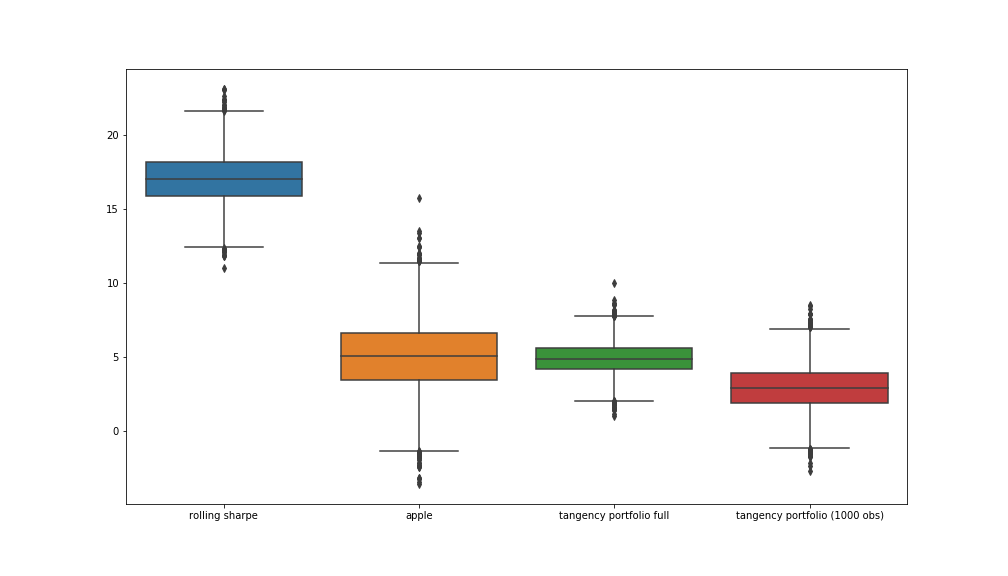
\includegraphics[scale=0.45]{figures/boxplot_monte_carlo.png}
\caption{Monte Carlo simulation - performance (in logs)}
\label{fig:logmontecarlo}
\end{figure}

Here we find again the rolling Sharpe algorithm performs best. The apple and tangency portfolio for the entire period seems to be doing approximately equal, comparing the mean, however, the variance is considerably lower for the tangency portfolio. Note the logarithmic \textit{y}-scale.
